\section{滞在ウォッチ}
% 屋内での在室・滞在状況の把握にはWi-Fi電波やユーザの移動時の加速度や角速度を用いたものなど様々な手法が提案されている．
屋内位置推定技術の応用として，在室管理や滞在状況の把握を目的としたシステムが数多く提案されている．
在室管理を目的としたシステムでは，人物の位置を高精度に推定する必要は必ずしもなく，部屋単位で人物の存在を把握できれば十分な場合も多い．
在室や滞在状況を推定する手法としては，ICカード\cite{ICcard}による入退室記録の取得，カメラやマイクを用いた映像・音声認識\cite{camera}\cite{voice}，無線電波を用いた自動検知\cite{WiFi}など，様々な方法が提案されている．
ICカードやチェックイン操作を用いる手法は在室判定の確実性が高い一方で，ユーザの操作忘れや誤操作が発生しやすい．
カメラによる顔認識や音声認識はユーザの追加操作を必要としない利点があるが，人の向きや遮蔽，環境音などの影響を受けやすく，プライバシの観点から導入が難しい場合もある．
一方，Wi-Fi や BLE などの無線電波を用いた手法は，ユーザの能動的な操作を必要とせず自動的に在室判定が可能である点で利便性が高いが，電池切れや電波環境，判定アルゴリズムの精度に依存するという課題がある．


以上の特徴から，部屋単位での位置推定ではBLE電波を用いる場合が多く，この研究でもBLE電波を用いた手法を採用している．
操作ミスや操作忘れが発生せず，常時精密な行動を監視する必要がなくプライバシに配慮される点は本手法の利点である．
また，在室人数の把握にとどまらず，個人を識別した在室・滞在管理が可能である点から，本手法を選択している．


BLE電波を用いた部屋単位の位置推定手法には，部屋に設置した物理ビーコンから電波を受信する方法\cite{BLE:EnvironmentBeacon}と，各ユーザが携帯する物理ビーコンの発する電波を部屋に設置した受信機で受信する方法\cite{BLE:UserBeacon}があり，このシステムでは後者を採用している．
前者は，特別な端末を携帯する必要がない一方で，自身のスマートフォンにアプリケーションをインストールする必要がある．
また，アプリケーションを常に稼働させる必要があるため，バッテリ消費量増大の懸念もある.
後者は，管理者から配布される物理ビーコンを用いているため持ち運び忘れや電池切れは発生しうるが，財布やカバンなどに入れ携帯するだけでよいのでユーザの負担を抑えられる．
他にも識別子が固定かつブロードキャスト送信されるため第三者から無断で追跡されるリスクがあるが，ビーコンから発信される識別子を定期的に更新する研究\cite{togawa}も行われている．


受信機は継続的に周囲のビーコン情報をサーバへと送信し，サーバがユーザと部屋の特定をする．
受信機には小型なマイクロコンピュータである Raspberry Pi\cite{RaspberryPi}が採用された．
Raspberry Pi は BLE 電波を継続的に受信し，ビーコンの識別子として UUID と受信機が持つ部屋の ID をサーバへ送信する．
サーバではデータベース内のユーザ情報や部屋情報と照らし合わせて特定される．
これにより，ユーザが自発的に行動を起こさずとも室内の人の検知が可能となる．
バッテリ消費を少なくするため物理ビーコンの発信間隔は最大値が採用され，サーバ負荷を抑えるためサーバへの送信頻度は数分おきとされた．
滞在情報はデータベースに保存され，現在の在室情報だけでなく過去の在室情報も管理している．


推定手法で特定されたユーザと部屋は，同じコミュニティのメンバのみに図\ref{fig:staywatch}のようなWebサイトで公開される．
リアルタイムで取得したデータをデータベースに保存，履歴化までを行っており，ブラウザで閲覧できるようになっている．
推定された現在の部屋ごとの滞在者一覧画面や，最新順に並んだ滞在履歴画面が確認できる．
また，グループのメンバの月ごとの総滞在時間を合算してランキングにし，競争心を喚起して来訪の促進を狙っている．
\begin{figure}[htb]
  \centering
  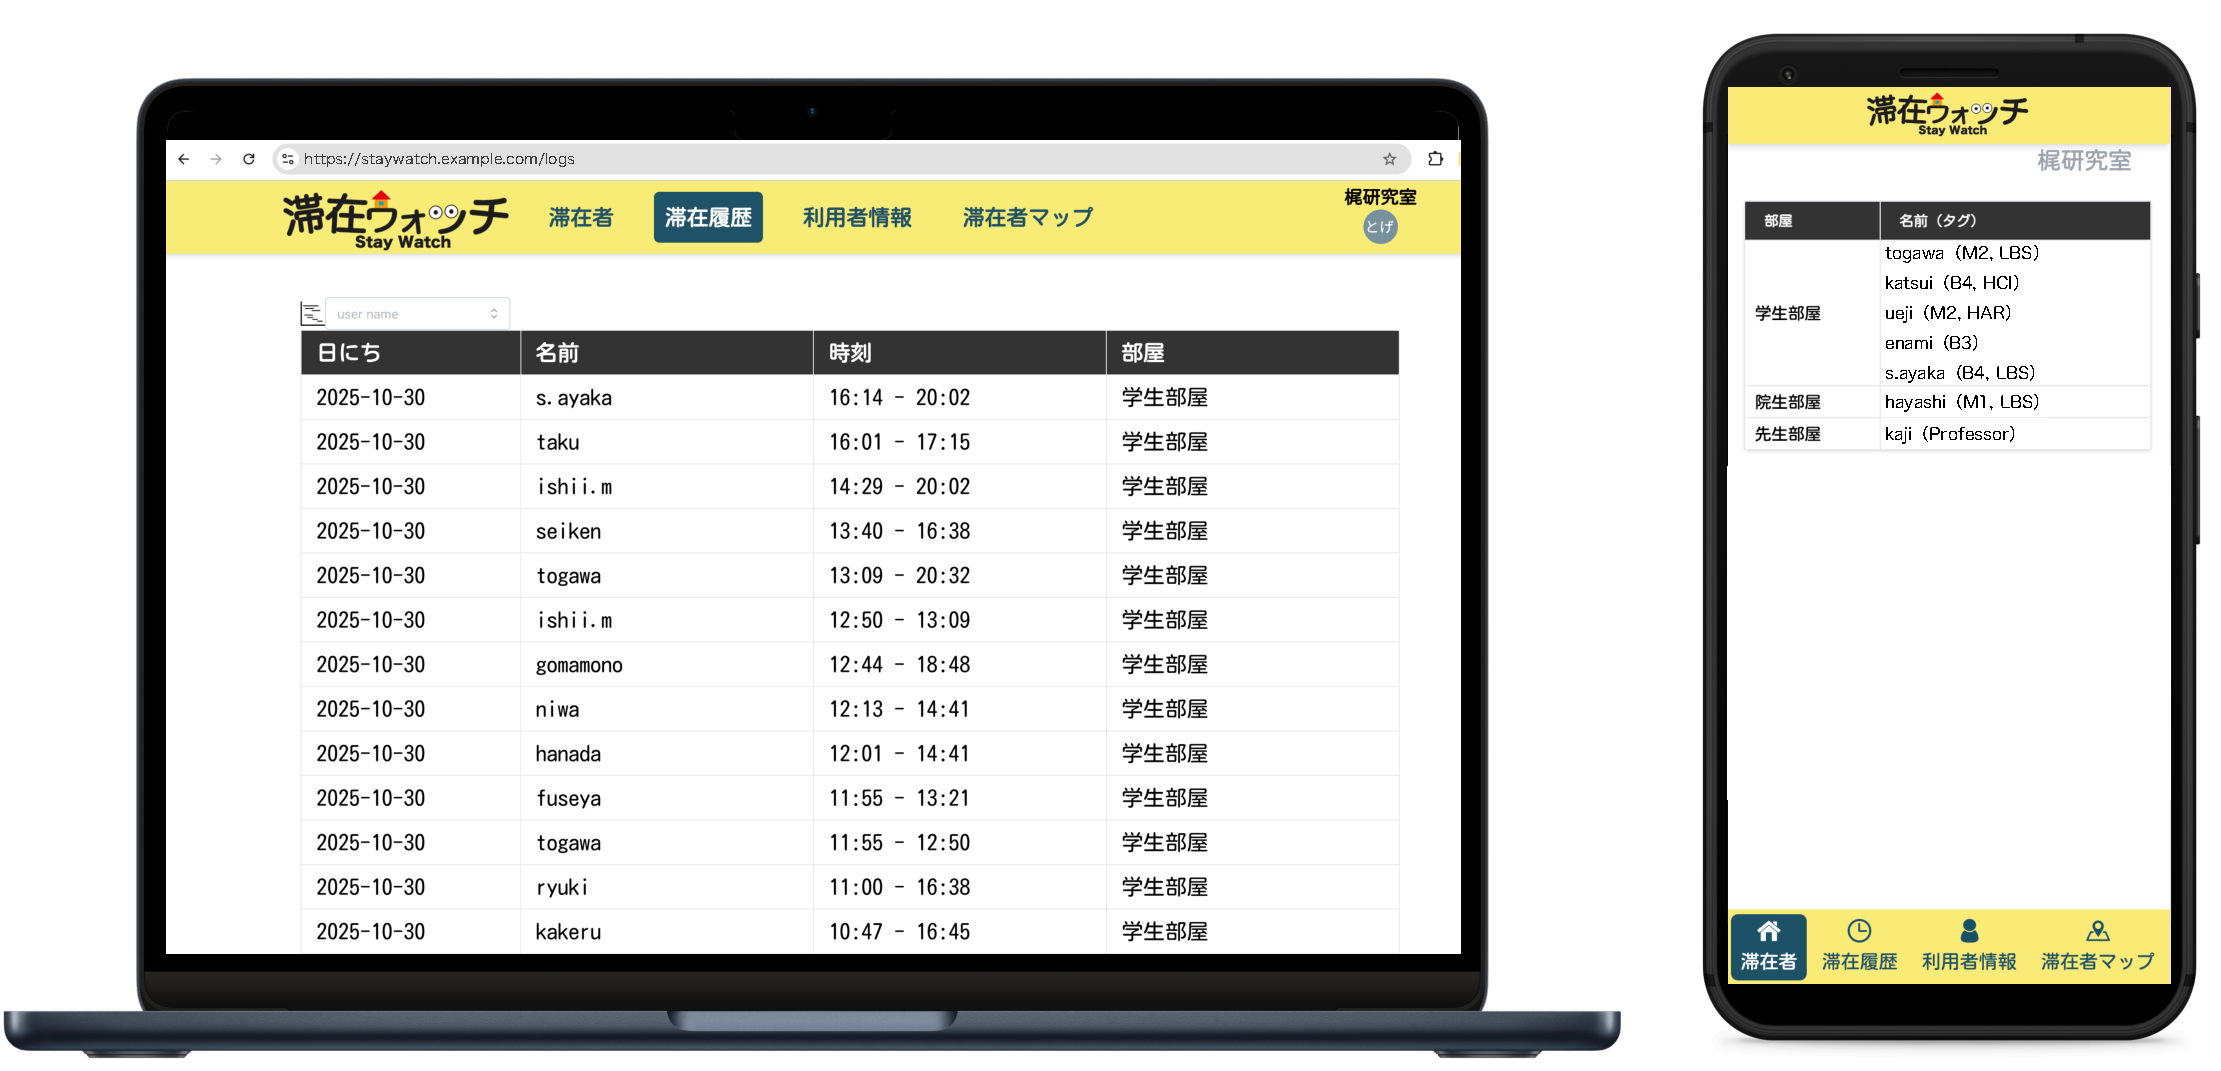
\includegraphics[width=0.8\linewidth]{fig/staywatch-display.pdf} % suzuki
  \caption{滞在ウォッチが提供するWebシステムの画面}
  \label{fig:staywatch}

\end{figure}


% APIでも提供されてるよがいる，これを3-3に繋げる
他にも，Web API を介して滞在情報が活用される状況が想定されている．
滞在情報の可視化や来訪者の通知，研究室への来訪促進といったシステムへの利用が検討されており，上記のWebサイトや次節に示す在室状況予測もこれにあたる．
滞在情報や過去の入退室記録をAPIとして提供する設計は，単一のアプリケーションに閉じた利用にとどまらず複数のサービスから柔軟に活用可能なプラットフォームとしての役割を果たす点に特徴がある．
% 他にも，先行研究では特定の人物の滞在状況の可視化やLINEと連携を行うアプリケーションが実装されている．
また，他アプリケーションとの連携を通して，ユーザが情報を閲覧する機会の増加を狙っている．